\documentclass[a4paper, 11pt]{article}
\usepackage{geometry}
\geometry{margin=2.5cm}

\usepackage[utf8]{inputenc}
\usepackage[T1]{fontenc}
\usepackage[english, magyar]{babel}
\usepackage{indentfirst}
\usepackage{enumitem}

% \usepackage{pythonhighlight}
\usepackage{graphicx}
\usepackage{float}

% Ábrakészítéshez
\usepackage{tikz}
\usetikzlibrary{fit, shapes.geometric}
\usepackage{fancyvrb}


\title{Evren}
\author{Bánovics-Angyal Gábor}

\begin{document}

\begin{titlepage}
	
	\raggedleft 
	
	\rule{1pt}{\textheight} 
	\hspace{0.05\textwidth} 
	\parbox[b]{0.75\textwidth}{
		{\Huge\bfseries Evren \\[0.5\baselineskip] \Large dokumentáció főbb működési elvekről}\\[2\baselineskip]
		{\large\textsc{Bánovics-Angyal Gábor}}
		
		\vspace{0.5\textheight}
		\hspace{8cm}
	}
\end{titlepage}
\pagebreak

%---------------------------------------------------------------------------------
%\tableofcontents

\section{A 3x3-as eltűnő jeles amőba}
A 3x3-as eltűnő jeles amőba (nemzetközi nevén gyakran Not Tictactoe vagy Infinite Tic-Tac-Toe) a klasszikus amőba (tic-tac-toe) egy izgalmas, pörgős változata. A játék lényege, hogy a táblán sosem alakulhat ki döntetlen, mert a jelek egy idő után eltűnnek.
\subsection*{Játékszabályok}
\subsubsection*{A játék célja}
Ugyanaz, mint a klasszikus amőbában: alakíts ki egy 3 elemű egyenest a saját jeledből vízszintesen, függőlegesen vagy átlósan.
\subsubsection*{Alapszabályok}
\begin{itemize}
    \item Kezdés: A játék egy üres, 3x3-as rácson indul. A játékosok felváltva teszik le a jeleiket \mbox{(x és $\circ$)}.
    \item Eltűnő jelek: Egy játékosnak legfeljebb 3 jele lehet egyszerre a táblán, ezért amikor lekerül a negyedik jel, a legrégebben lerakott jel azonnal eltűnik.
\end{itemize}






\section{Program célja}
\indent A program egy hibavezérelt, visszacsatoláson alapuló megerősítéses tanulási modellt alkalmaz. A mérkőzések során a szoftver nyilvántartja a táblaállásokhoz tartozó lehetséges lépéseket. Amennyiben egy játszma vereséggel végződik, a program a legutolsó lépést hibás döntésnek minősíti, és az adott konkrét táblaállásban eltávolítja a választható opciók közül (vagyis tiltólistára helyezi). Ennek köszönhetően a jövőben, ha pontosan ugyanez a pozíció előáll, a program elkerüli a közvetlen vesztést okozó döntést, fokozatosan leszűkítve a lehetséges lépéseket.

\section{Megoldandó problémák}
\indent A legfontosabb megoldandó probléma, hogy egy bizonyos állás 8-féleképpen állhat elő (az összes lehetséges transzformációt figyelembe véve). Vagyis ha a gyakorlatilag egyforma eseteket nem különítjük el, akkor a programnak 8-szor annyit kell tanulnia. A megoldás kulcsa, hogy minden egyes táblaálláshoz egy egyértelműen előállítandó tájolást határozok meg. \\
\indent Ennek módszere a következő:
\begin{enumerate}
    \item A jeleket számokkal helyettesítjük, hogy számon lehessen tartani, hogy melyik a legöregebb. A számok kettő hatványok lesznek, mert összegeket képzünk belőlük, és a cél, hogy egy bizonyos összeg pontosan egyféleképpen állhasson elő. Továbbá 2-től kezdjük a számozást, mert az 1-est fenntartjuk érvényes lépés jelölésére egy üres mezőben.
        \begin{itemize}
            \item $\circ$: 2, 4, 8
            \item x: 16, 32, 64
        \end{itemize}

    \pagebreak
    \item A 3x3-as tábla mind a 4 2x3-as blokkjában meghatározzuk a jelek számértékeinek összegét. Ezt követően a táblát úgy fogjuk forgatni, hogy a legnagyobb összeggel rendelkező blokk a felső 2x3-as helyre kerüljön.\\
    Ábra:
        \begin{center}
            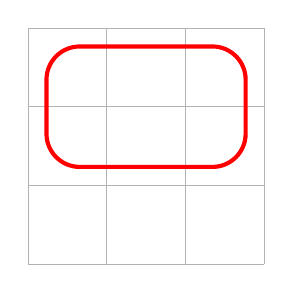
\begin{tikzpicture}[scale=1]
                % 1. A 3x3-as rács kirajzolása
                \draw[step=1cm, gray!60, very thin] (0,0) grid (3,3);
            
                % 2. Mezők elhelyezése és elnevezése (c-oszlop-sor formában)
                % A koordináta-rendszer alulról felfelé megy: y=0..2, x=0..2
                % Így az y=2 a legfelső sor, az y=1 a középső, az y=0 a legalsó
                \foreach \x in {0,1,2} {
                    \foreach \y in {0,1,2} {
                        \node (c-\x-\y) at (\x+0.5, \y+0.5) {};
                    }
                }
            
            
                % 3. Az ovális / lekerekített karikázás a felső 2x3-as részre (y=1 és y=2 sorok)
                \node[
                    draw=red,               % Keret színe
                    line width=1.5pt,       % Vastagság
                    rounded corners=12pt,   % Ettől lesz szép lekerekített / ovális hatású
                    fit=(c-0-1) (c-2-2),    % Bal alsó (0,1) és jobb felső (2,2) cellák közrezárása
                    inner sep=4pt           % Mennyi hely maradjon a tartalom és a keret között
                ] {};
            \end{tikzpicture}
        \end{center}
        
    \item Az így felülre forgatott 2x3-as blokknak összegezzük a bal- és jobb oldali 2x2-es blokkjait, majd úgy tükrözzük az adott állást, hogy a nagyobb összegű blokk a bal felső 2x2-es legyen. \\
    Ábra:
    \begin{center}
        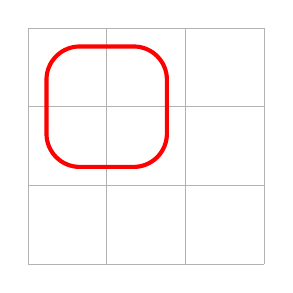
\begin{tikzpicture}[scale=1]
            % 1. A 3x3-as rács kirajzolása
            \draw[step=1cm, gray!60, very thin] (0,0) grid (3,3);
        
            % 2. Mezők elhelyezése és elnevezése (c-oszlop-sor formában)
            \foreach \x in {0,1,2} {
                \foreach \y in {0,1,2} {
                    \node (c-\x-\y) at (\x+0.5, \y+0.5) {};
                }
            }
        
        
            % 3. Karikázás
            \node[
                draw=red,               
                line width=1.5pt,       
                rounded corners=12pt,   
                fit=(c-0-1) (c-1-2),    
                inner sep=4pt           
            ] {};
        \end{tikzpicture}
    \end{center}
\end{enumerate}

\indent Mivel a jeleket 2 hatványokkal kódoltuk, ezért egy összeg felfogható egy 2-es számrendszerben felírt számnak, vagyis egy bizonyos összeg pontosan egyféleképpen állítható elő. Ezért két blokk összege csak akkor lehet egyenlő, ha ugyanazok a számok szerepelnek bennük. Ami viszont a maximális 6 jel esetében nem lehetséges, mert két 2x3-as blokknak legfeljebb 3 közös eleme lehet. Továbbá a 3. lépésben a 2x2-es blokkok sem lehetnek egyforma összegűek, mert egy 2x3-as blokkba legalább 3 jelnek bele kell esnie, és két 2x2-es blokknak csak 2 közös eleme van, vagyis biztosan lesz valamelyik blokkban még legalább egy szám, ami nem a kettejük metszetébe esik. Vagyis ez a módszer a 6 jeles állásokhoz egy egyértelmű tájolást rendel hozzá. \\
\indent További megfontolást igényelnek azok az esetek, amikor még nincs letéve mindkét játékos mindhárom jele. Ezekben az esetekben lehetségesek olyan esetek, amikor több egyforma összegű 2x3-as blokkok vannak. Ekkor meghatározzuk mind a négy 2x2-es blokk összegét, amelyek közül kiválasztjuk az első legnagyobbat (mert még itt is lehet több egyforma), és a táblát a 3. pontnak megfelelően úgy forgatjuk, hogy a bal felső sarokba essen. Ezután megvizsgáljuk az ábrán jelölt két mező értékét és szükség szerint tükrözzük, hogy a felső középső elem legyen a nagyobb. \\
Ábra:
    \begin{center}
        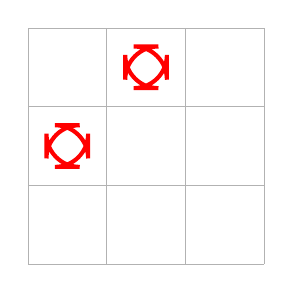
\begin{tikzpicture}[scale=1]
            % 1. A 3x3-as rács kirajzolása
            \draw[step=1cm, gray!60, very thin] (0,0) grid (3,3);
        
            % 2. Mezők elhelyezése és elnevezése (c-oszlop-sor formában)
            \foreach \x in {0,1,2} {
                \foreach \y in {0,1,2} {
                    \node (c-\x-\y) at (\x+0.5, \y+0.5) {};
                }
            }
        
        
            % 3. Karikázás
            \node[
                draw=red,               
                line width=1.5pt,       
                rounded corners=12pt,   
                fit=(c-0-1) (c-0-1),    
                inner sep=4pt           
            ] {};
            \node[
                draw=red,               
                line width=1.5pt,       
                rounded corners=12pt,   
                fit=(c-1-2) (c-1-2),    
                inner sep=4pt           
            ] {};
        \end{tikzpicture}
    \end{center}
Így szintén egy egyértelmű tájolást sikerült elérni.



\pagebreak
\subsection{Transzformálás}
\indent A táblaállást egy 9 elemű sorvektorként kezelem (szükség esetén másolást követően 3x3-as mátrixszá alakítom és úgy dolgozok vele tovább), így egy transzformáció megfeleltethető egy 9x9-es mátrixszal való szorzásnak. Az egységes tájolásra traszformálást jobbról való szorzásnak veszem, így a visszatranszformálás egy ugyanazzal a mátrixszal való balról (oszlopvektort) való szorzás lesz. \\
\indent Ezek a transzformációk, a tájolás megkeresése, valamint a táblatranszformálás a \mbox{\emph{transformations.py}} file-ban találhatók meg.



\subsection{Szimmetriák kezelése}
\indent Mivel az egyes jelek nem egyforma értékűek, így a maximális 6 jel esetében nem alakulhat ki szimmetrikus állás. Viszont az első három jel rakása esetén még igen. Mivel az egységes tájolást úgy végezzük, hogy a felső 2x3-as illetve a bal felső 2x2-es blokkhoz viszonyítunk mindent, így a szimmetriákat arra a két esetre kell megvizsgálnunk (az egységes tájolásra transzformálás után), hogy a függőleges szimmetriatengelyre, illetve a főátlóra nézve szimmetrikus-e az adott állás. Amennyiben:
\begin{itemize}
    \item Függőleges tengelyre szimmetrikus: a jobb oldali oszlopban levő mezőket kivesszük a választandó lehetőségek közül
    \item Főátlóra szimmetrikus: csak a felső háromszögben levő mezők lesznek választható mezők
\end{itemize}
Természetesen csak a szabad mezőket korlátozzuk.  Ezt az \mbox{\emph{ai\_if\_symmetrical}} függvény végzi.\\
Ezzel az utolsó lehetőséget is kiszűrtük, hogy egyforma lépéseket külön esetként vizsgáljon.


\subsection{Lehetséges lépések terének csökkentése}
\indent Minden esetben csak 3 lehetséges lépése van (tanulás útján való kizárás nélkül), azonban vannak esetek, amikor egyértelmű a nyerő lépés. Mivel minden lépés során a legrégebbi jel eltűnik, ezért a nyerő lépés vizsgálatánál a táblát kezdettől fogva úgy vizsgáljuk, hogy a legrégebbi jelet (amelyik szemszögéből vizsgáljuk) kitöröljük, majd megvizsgáljuk, hogy valamelyik sorban, oszlopban vagy átlóban van-e olyan szabad hely, amellyel 3 egyforma jelet lehet kialakítani.
Ezt az \mbox{\emph{if\_force\_win}} függvény végzi.\\
Ennél több taktikai lépés beépítése történt és nem is szükséges.




\section{Állás elmentése}
\indent Az egyes állásokat az egységes tájolásra transzformált állapotban mentjük el, úgy, hogy a táblaállásnak megfelelő számokat folytonosan egy string-be írjuk (az üres helyeket 0-val jelölve). Az adott álláshoz tartozó tiltott lépéseket halmazban tároljuk. Ebből a két adatszerkezetből képzünk egy szótárat. \\
\indent File-ba írás esetén kiírjuk a stringet (kulcs) a következő sorba a hozzá tartozó tiltott lépések koordinátáit egymás mellé, mivel úgyis csak egyjegyű számok lehetnek (0-tól 8-ig).





\pagebreak
\section{Számításigény felmérése}
\indent Számításigény felméréséhez először határozzuk meg, hogy mennyi táblaállás lehetséges. Összesen 9 mezőből mindig 6 foglalt jelekkel, ez ${9 \choose 6}$ féleképpen lehetséges, és a kiválasztott 6 elemet még $6!$ féleképpen permutálhatjuk egymás között. Továbbá minden táblaállást 8-szor számoltunk. Így adódik
\begin{equation}
    \frac{9!}{6!\cdot3!} \cdot 6! \cdot \frac{1}{8} = 7560
\end{equation}

Amihez még hozzájönnek az 5, 4, 3, 2 és 1 jeles állások számai, de a nagyságrendet jól tükrözi ez a szám.





\section{Statisztika}
\indent A számítógépes játék során egy bizonyos lépésszám fölött ($1000$) már leállítjuk a játékot, hogy ne vigyen el egy játék véletlenül sok időt. Statisztika készítése során mérem, hogy egy bizonyos játékszám ($200$) során összesen mennyi lépés, mennyi megszakítás történt, mennyi ideig tartott, a gép összesen mennyi lépés közül választott az adott intervallumban, valamint ebből képzünk egy arányt is az összes lépésszámmal. \\
\indent Mindezek közül e legutóbbi a leginformatívabb:
\begin{figure}[H]
    \centering
    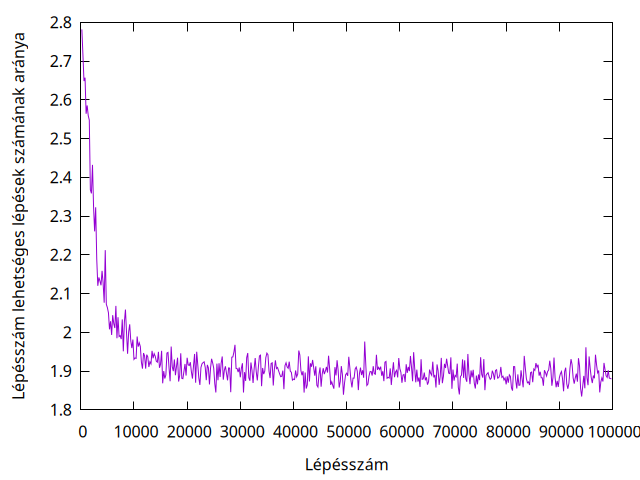
\includegraphics[width=0.5\linewidth]{ratio.png}
    \caption{Arányszám}
    \label{fig:placeholder}
\end{figure}
Az ábrából az látszik, hogy 100.000 parti lejátszása után már a szimuláció előrehaladásával egy vizsgált játékintervallumon belül a ténylegesen megtett lépések száma és a meglátogatott állások során vizsgált összes lehetséges lépés számának aránya 2 alá csökkent, vagyis körülbelül 20.000 parti után már majdnem minden állásban van egy olyan lépés, amit kizárhat. Viszont további 4-szer annyi szimulációt futtatva ez az arány tovább már nem csökkent, amiből arra lehet következtetni, hogy a játékban nincs nyerő lépése a kezdő félnek. Ugyanakkor az 1000 lépéses határt egyetlenegyszer sem lépte át, amit a következő ábrán láthatunk:
\begin{figure}[H]
    \centering
    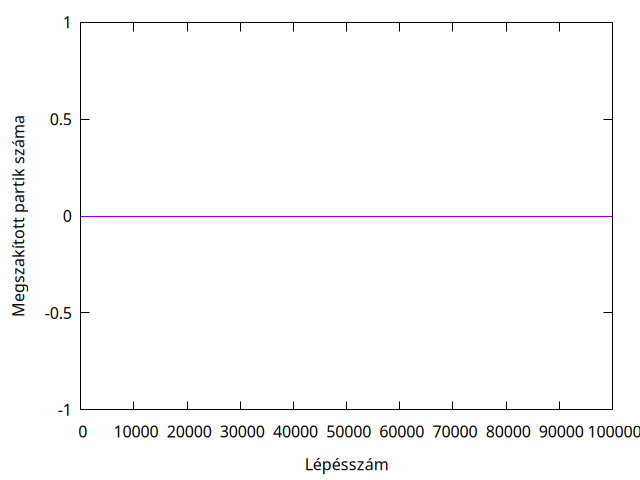
\includegraphics[width=0.5\linewidth]{break.png}
    \caption{1000 lépést meghaladó, emiatt megszakított partik száma}
    \label{fig:placeholder}
\end{figure}




\end{document}
